
\begin{figure}[t]
\centering
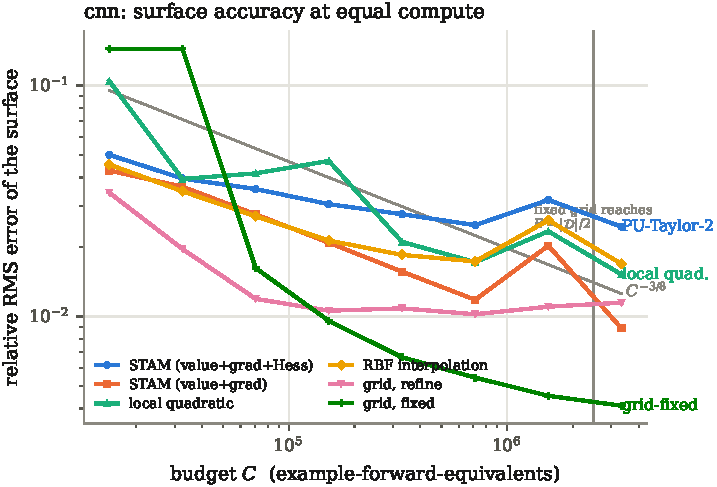
\includegraphics[width=0.72\linewidth]{../figures/budget_error_cnn.pdf}
\caption{Relative RMS error of the rendered surface against compute budget (CNN/CIFAR-10, median of three seeds, log--log). The two grid baselines flatten: they interpolate their own noise, so past a point extra budget buys nothing (\Cref{prop:floor}). The guide line is the predicted $C^{-3/8}$.}
\label{fig:budget}
\end{figure}


\begin{figure}[t]
\centering
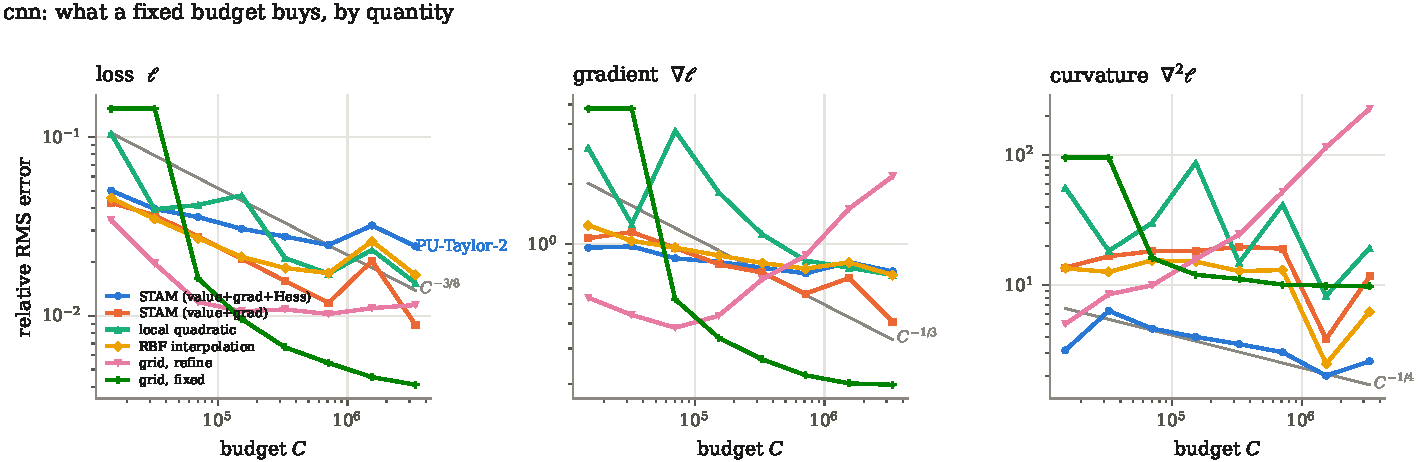
\includegraphics[width=\linewidth]{../figures/rate_separation_cnn.pdf}
\caption{The same sweep scored on three quantities. Derivative probing does not improve the rate for the surface, only its constant --- but it strictly improves the rate for the gradient field and for curvature, which is what \Cref{tab:rates} predicts and what practitioners read off these figures.}
\label{fig:rates}
\end{figure}


\begin{figure}[t]
\centering
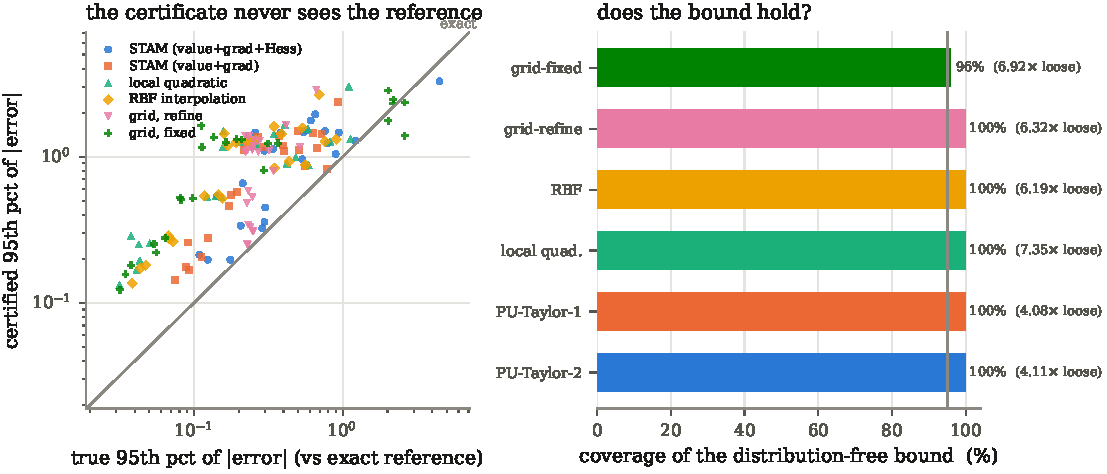
\includegraphics[width=\linewidth]{../figures/certificate_cnn.pdf}
\caption{Left: the certified error against the true error measured against the exact reference. The certificate never sees the reference. Right: empirical coverage of the $95\%$ upper bound, and how tight it is.}
\label{fig:cert}
\end{figure}


\begin{figure}[t]
\centering
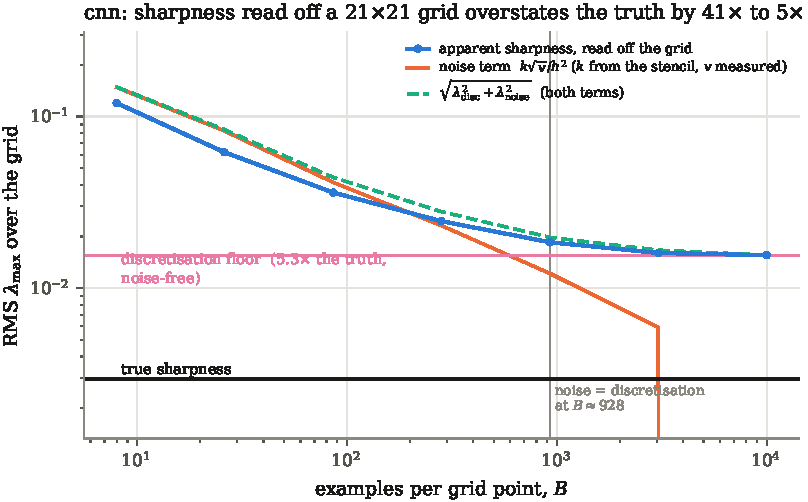
\includegraphics[width=0.68\linewidth]{../figures/sharpness_cnn.pdf}
\caption{Sharpness read off a fixed grid, against the per-point sample size. The apparent value never falls below the noise floor $\lambda_{\mathrm{noise}}\propto\sigma/(h^2\sqrt B)$, whose constant comes from the second-difference stencil and is not fitted. At sample sizes typical of a landscape figure the floor exceeds the signal.}
\label{fig:sharp}
\end{figure}


\begin{figure}[t]
\centering
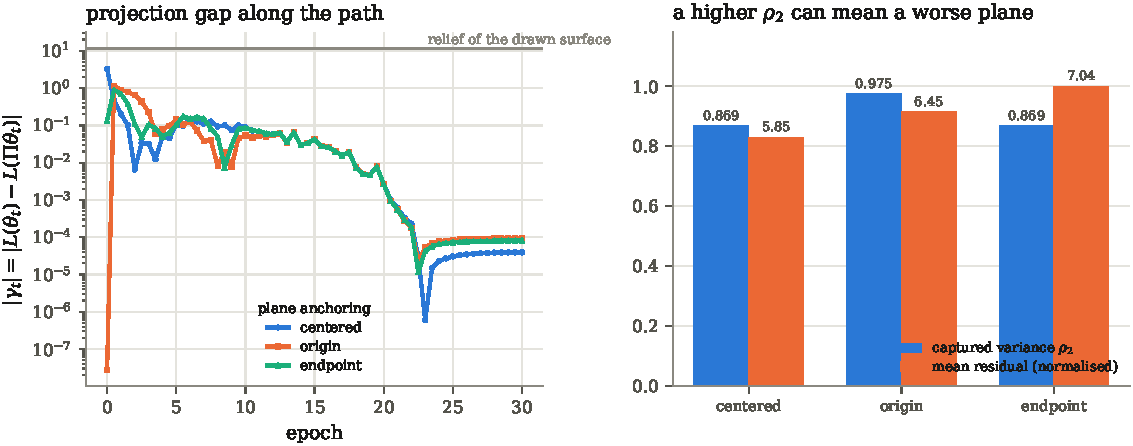
\includegraphics[width=\linewidth]{../figures/fidelity_cnn.pdf}
\caption{Left: the projection gap along the optimiser's path, for three plane constructions. Right: the $\theta_0$-anchored plane reports the highest $\rho_2$ and has the largest residual.}
\label{fig:fid}
\end{figure}


\begin{figure}[t]
\centering
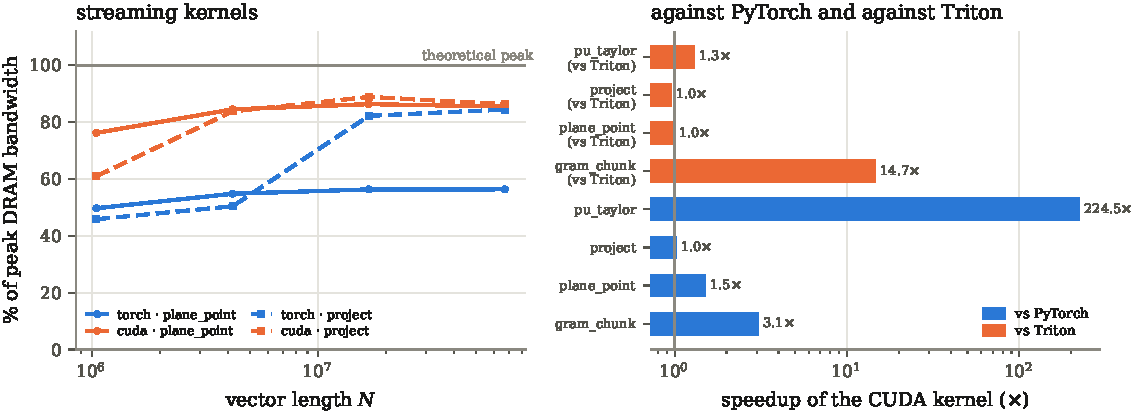
\includegraphics[width=\linewidth]{../figures/kernels.pdf}
\caption{Left: achieved fraction of peak DRAM bandwidth for the two streaming kernels. Right: speedup of the hand-written CUDA kernels over PyTorch and over the Triton implementations.}
\label{fig:kernels}
\end{figure}


\begin{figure}[t]
\centering
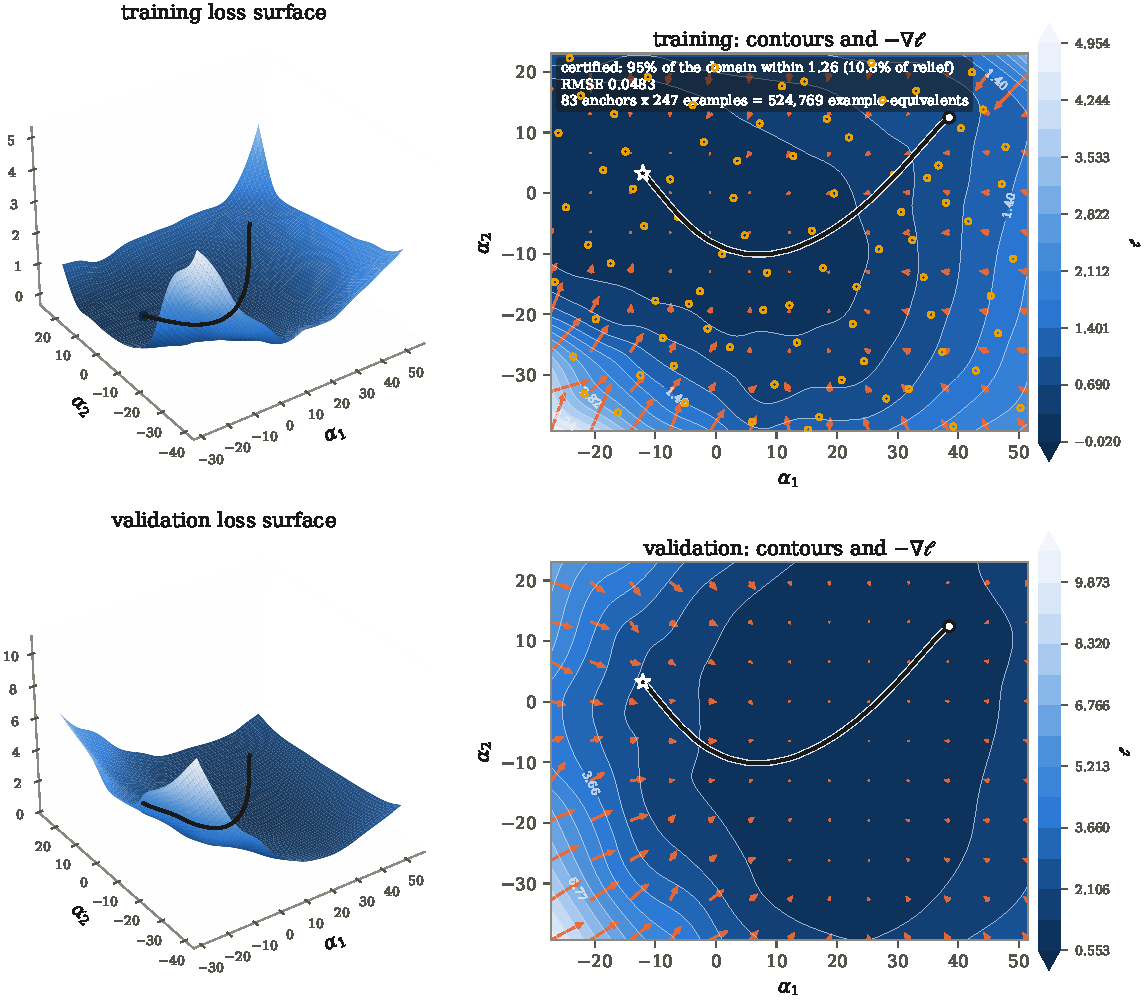
\includegraphics[width=\linewidth]{../figures/landscape_cnn.pdf}
\caption{A certified landscape (CNN/CIFAR-10). Contour intervals are set to at least twice the certified RMS error, so no contour is drawn that the measurement cannot resolve. The quiver field is the exact gradient of the surface, computed analytically from \eqref{eq:pugrad}. Open circles mark the anchors actually probed.}
\label{fig:landcnn}
\end{figure}


\begin{figure}[t]
\centering
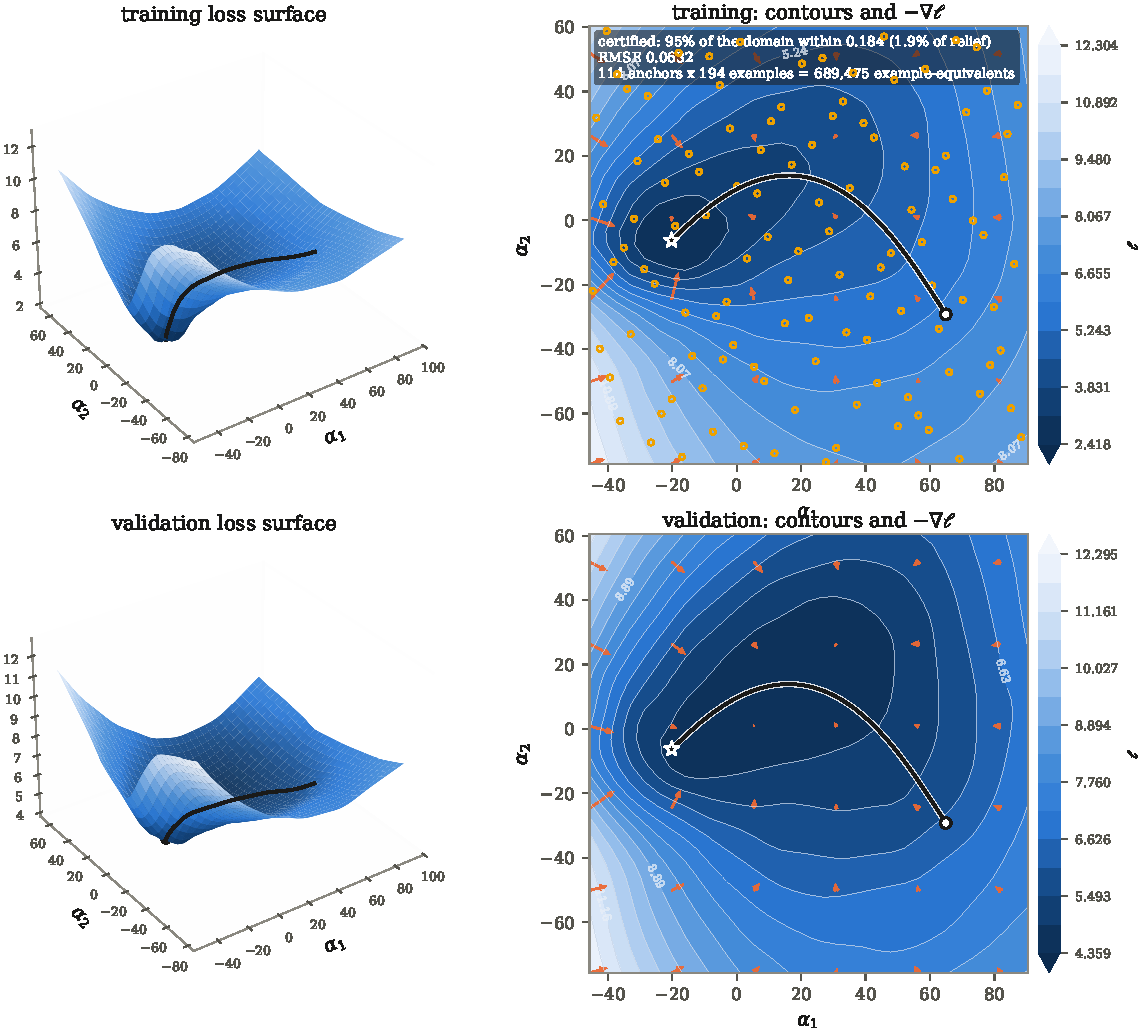
\includegraphics[width=\linewidth]{../figures/landscape_gpt.pdf}
\caption{A certified landscape for the \GPTparams-parameter transformer on WikiText-2.}
\label{fig:landgpt}
\end{figure}


\begin{figure}[t]
\centering
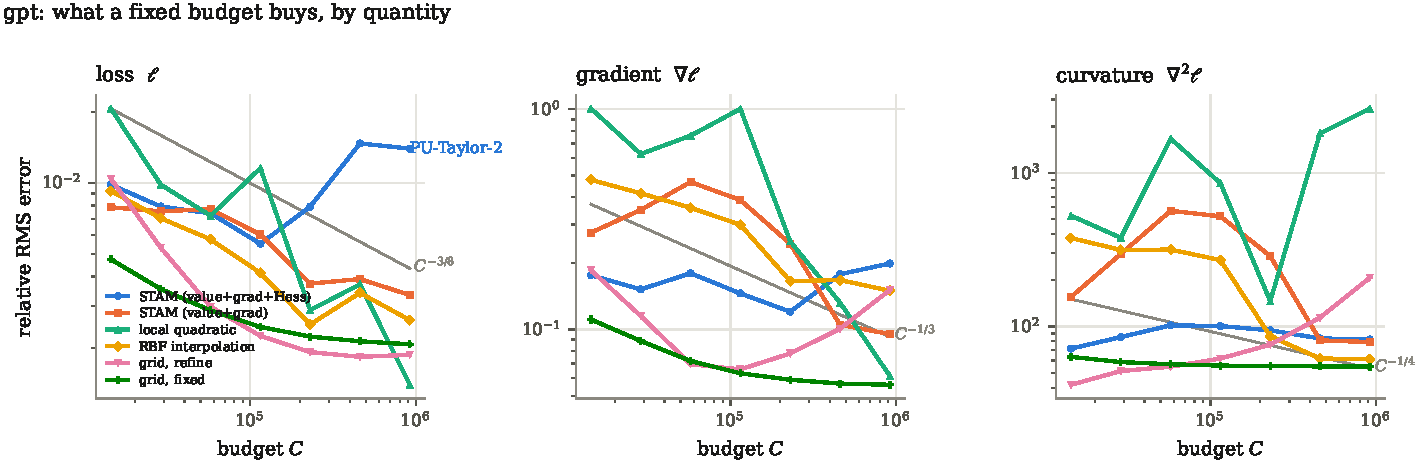
\includegraphics[width=\linewidth]{../figures/rate_separation_gpt.pdf}
\caption{The same sweep on the \GPTparams-parameter transformer. The grid-refinement baseline again degrades with budget on curvature. The relative curvature metric discriminates poorly here because the true curvature is small over a domain where the loss saturates near $\ln|V|$ --- a limitation of the subject, stated in \Cref{sec:limits}.}
\label{fig:ratesgpt}
\end{figure}


\begin{figure}[t]
\centering
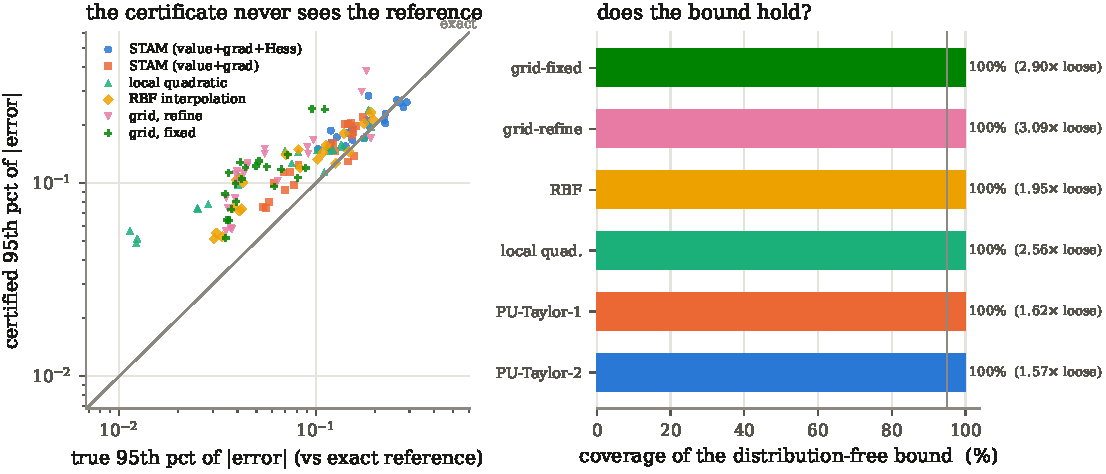
\includegraphics[width=\linewidth]{../figures/certificate_gpt.pdf}
\caption{Certificate validity on the transformer. The error field is far less heavy-tailed than the CNN's, and the certified point estimate is correspondingly close to the truth.}
\label{fig:certgpt}
\end{figure}


\begin{figure}[t]
\centering
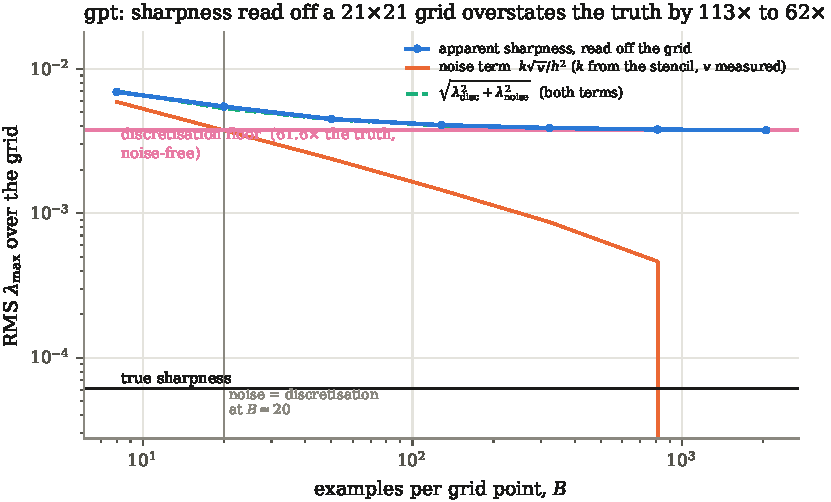
\includegraphics[width=0.68\linewidth]{../figures/sharpness_gpt.pdf}
\caption{Sharpness read off a grid for the transformer: overstated by \GPTsharpworst$\times$ at small samples and still \GPTsharpfloor$\times$ when the probe is exact.}
\label{fig:sharpgpt}
\end{figure}


\begin{figure}[t]
\centering
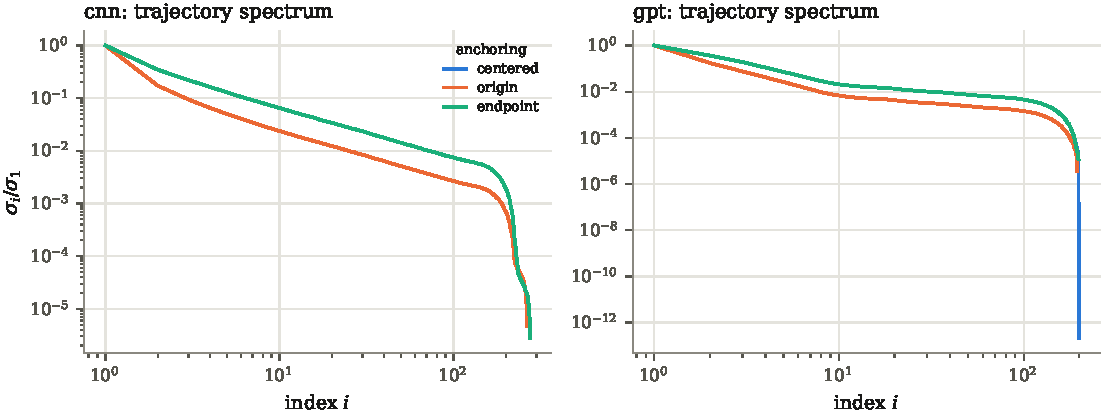
\includegraphics[width=\linewidth]{../figures/spectrum.pdf}
\caption{Trajectory spectra. The uncentred construction concentrates more of \emph{its} ratio in the leading pair, which is why $\rho_2$ favours it while the residual does not.}
\label{fig:spectrum}
\end{figure}


\begin{figure}[t]
\centering
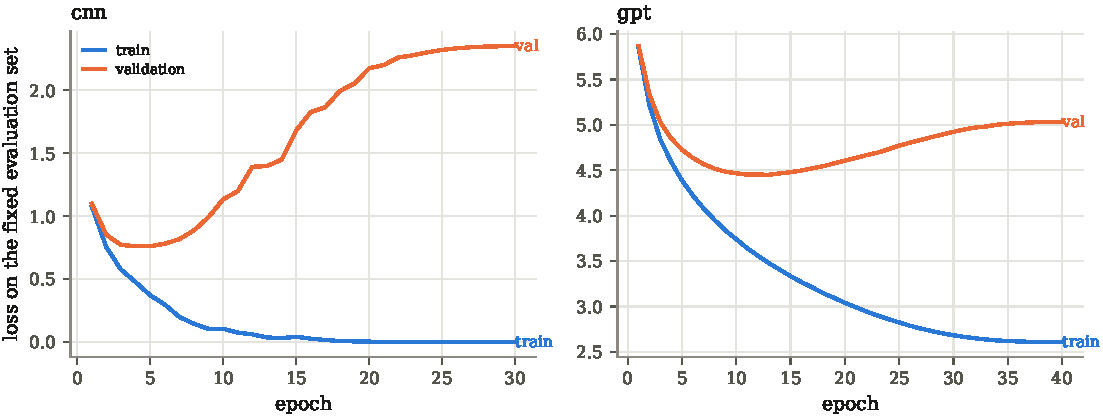
\includegraphics[width=\linewidth]{../figures/training.pdf}
\caption{Training curves on the fixed evaluation sets that define the landscapes.}
\label{fig:training}
\end{figure}
